\documentclass[12pt]{article}
\usepackage[utf8]{inputenc}
\usepackage[T1]{fontenc}
\usepackage{geometry}
\usepackage{amsmath}
\usepackage{amssymb}
\usepackage{enumitem}
\usepackage{indentfirst}
\usepackage{xcolor}
\usepackage{graphicx}
\usepackage{fancyhdr}
\usepackage[spanish]{babel}
\usepackage{float} % Added for [H] specifier to force figure placement

% Set margins
\geometry{a4paper, margin=1in}

% Specify path to img folder
\graphicspath{{img/}}

\pagestyle{fancy}
\fancyhf{} 
\fancyhead[L]{Simulación de la Centralita Telefónica de la Compañía de Seguros “La Otra Vida”}
\renewcommand{\headrulewidth}{0.4pt} 
\setlength{\headheight}{15pt}

% Customize section headings
\renewcommand{\thesection}{\arabic{section}}
\renewcommand{\thesubsection}{\arabic{section}.\arabic{subsection}}
\renewcommand{\thesubsubsection}{\arabic{section}.\arabic{subsection}.\arabic{subsubsection}}

% Set paragraph indentation and spacing
\setlength{\parindent}{1em}
\setlength{\parskip}{0.5em}

% Custom list formatting
\setlist[itemize]{leftmargin=2em}
\setlist[enumerate]{leftmargin=2em}

\title{Simulación de la Centralita Telefónica de la Compañía de Seguros “La Otra Vida”}
\author{Salma Fonseca Curbelo C-312}

\begin{document}

\maketitle
\newpage

\section{Introducción}

\subsection{Descripción del proyecto}
Este proyecto consiste en la simulación de una centralita telefónica de la compañía de seguros “La Otra Vida”. El sistema recibe llamadas de clientes que requieren atención para reclamaciones o solicitud de información, procesadas una a una a través de un contestador automático que lleva a la cola del servicio solicitado.

\subsection{Objetivos y metas}
El objetivo principal es determinar el tamaño y el tiempo promedio de las colas en cada servicio del sistema (contestador automático, reclamaciones e información), así como la utilización de los servidores y el tiempo que pasa el cliente desde el inicio de la llamada hasta que termina de ser atendido.

\subsection{Sistema a simular y variables de interés}
El sistema se compone de:
\begin{enumerate}
    \item Contestador automático: Recibe todas las llamadas (tasa de llegada de 35 por hora, distribución de Poisson) y procesa la decisión del cliente (tiempo medio de 30 segundos, distribución exponencial). Solo un cliente puede ser atendido a la vez, con una cola para los que esperan.
    \item Nodo de reclamaciones: Con 3 servidores en paralelo, atiende el 55\% de las llamadas iniciales con un tiempo medio de servicio de 6 minutos (exponencial). El 2\% de estas llamadas se redirigen al nodo de información.
    \item Nodo de información: Con 7 servidores en paralelo, atiende el 45\% restante de las llamadas iniciales con un tiempo medio de servicio de 20 minutos (exponencial). El 1\% de estas llamadas se redirigen al nodo de reclamaciones.
\end{enumerate}

Variables de interés:
\begin{itemize}
    \item Tamaño promedio de las colas en cada nodo (contestador, reclamaciones, información).
    \item Tiempo medio que un cliente pasa en el sistema.
    \item Tiempos de espera en cola por nodo.
    \item Utilización de los servidores.
    \item Distribución de las trayectorias de los clientes.
\end{itemize}

\subsection{Variables que describen el problema}
\begin{itemize}
    \item Tasa de llegada: $\lambda = 35$ llamadas por hora (Poisson).
    \item Tiempo de decisión en el contestador: Media de 30 segundos (exponencial).
    \item Probabilidad de reclamaciones: 55\% (botón 1).
    \item Probabilidad de información: 45\% (botón 2).
    \item Tiempo de servicio en reclamaciones: Media de 6 minutos (exponencial), con 3 servidores.
    \item Tiempo de servicio en información: Media de 20 minutos (exponencial), con 7 servidores.
    \item Probabilidad de redirección:
    \begin{itemize}
        \item De reclamaciones a información: 2\%.
        \item De información a reclamaciones: 1\%.
    \end{itemize}
\end{itemize}

\section{Detalles de Implementación}
La simulación se implementó utilizando un enfoque de simulación por eventos discretos. Los pasos seguidos fueron:
\begin{enumerate}
    \item Definición de la clase \texttt{InsuranceCallCenterSimulation}:
    \begin{enumerate}
        \item Se inicializaron parámetros como la tasa de llegada, funciones para tiempos de servicio y duración de la simulación (24 horas).
    \end{enumerate}
    \item Gestión de eventos:
    \begin{enumerate}
        \item Se definieron cuatro tipos de eventos: llegada de llamada (\texttt{call\_arrival}), fin de atención en el contestador (\texttt{end\_answer}), fin de servicio en reclamaciones (\texttt{end\_claim}) y fin de servicio en información (\texttt{end\_info}).
        \item Los eventos se almacenan en una cola de prioridad ordenada por tiempo.
    \end{enumerate}
    \item Procesamiento de colas y servidores:
    \begin{enumerate}
        \item Contestador: Una cola para las llamadas entrantes y un único servidor. Si está ocupado, las nuevas llamadas esperan.
        \item Reclamaciones: Una cola y tres servidores. Las llamadas se asignan a un servidor que no esté ocupado; si todos lo están, se agregan a la cola.
        \item Información: Siete servidores que trabajan en paralelo, es decir hay una cola única, con lógica similar.
        \item Se implementó el flujo que siguen los clientes entre servicios acorde con las probabilidades que se proporcionaron al enunciar el problema.
    \end{enumerate}
    \item Recopilación de estadísticas:
    \begin{enumerate}
        \item Se registraron los tiempos de llegada, inicio y fin de cada etapa, así como las longitudes de las colas en cada evento.
        \item Se calcularon métricas como el tiempo en el sistema, tiempos de espera, utilización de servidores y distribución de trayectorias.
    \end{enumerate}
    \item Ejecución y visualización:
    \begin{enumerate}
        \item La simulación se ejecutó durante 24 horas simuladas.
        \item Se generaron histogramas, diagramas de caja y gráficos de barras para analizar las variables de interés.
    \end{enumerate}
\end{enumerate}

\section{Resultados y Experimentos}

\subsection{Hallazgos de la simulación}
La simulación proporcionó las siguientes métricas promedio:
\begin{itemize}
    \item Tamaño promedio de la cola en el contestador es de 0 llamadas.
    \begin{figure}[H]
        \centering
        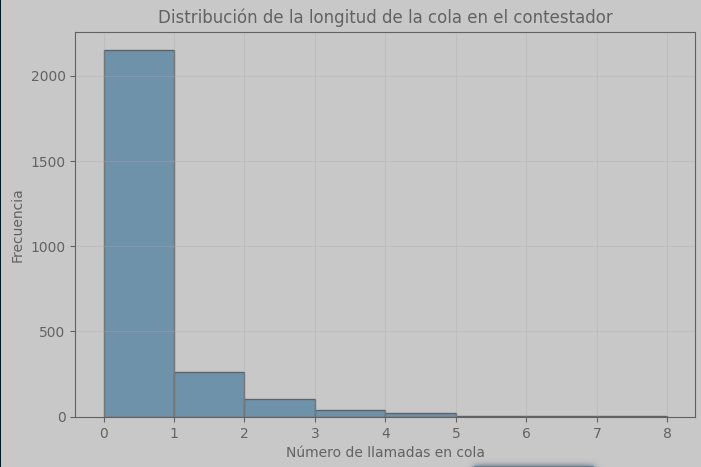
\includegraphics[width=0.8\textwidth]{Answ_queue.png}
        \caption{Tamaño de la cola del contestador}
        \label{fig: Tamaño de la cola del contestador}
    \end{figure}
    \item Tamaño promedio de la cola en las reclamaciones es entre 0 y 1 llamada.
    \begin{figure}[H]
        \centering
        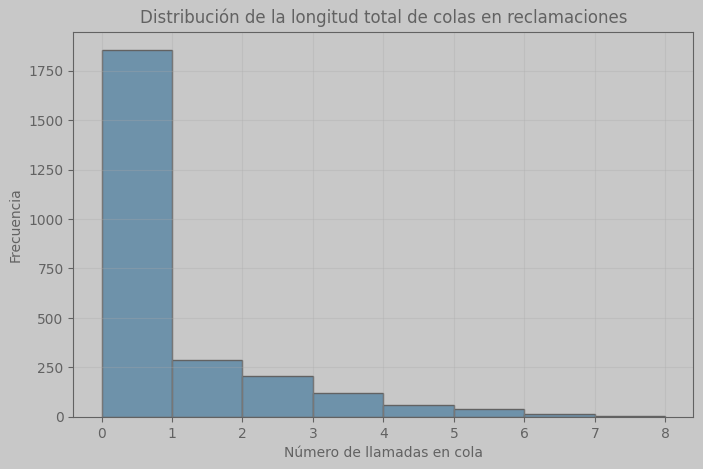
\includegraphics[width=0.8\textwidth]{claim_queue.png}
        \caption{Tamaño de la cola de reclamación}
        \label{fig: Tamaño de la cola de reclamación}
    \end{figure}
    \item Tamaño promedio de la cola en información es entre 0 y 1 llamada.
    \begin{figure}[H]
        \centering
        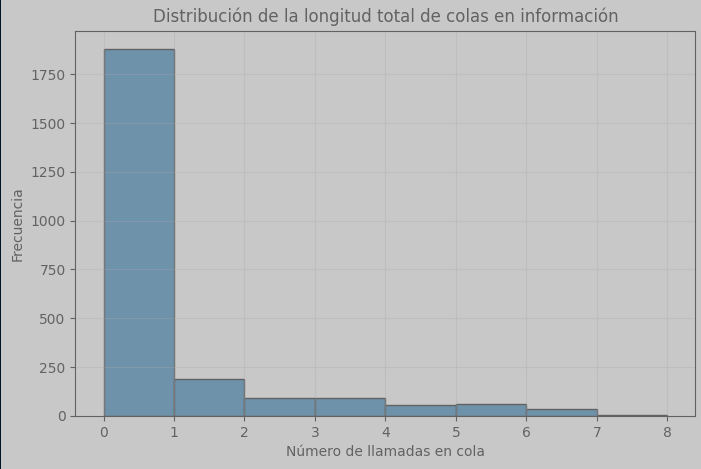
\includegraphics[width=0.8\textwidth]{info_queue.png}
        \caption{Tamaño de la cola de información}
        \label{fig: Tamaño de la cola de información}
    \end{figure}
    \item Los tiempos de espera en minutos del contestador, reclamaciones e información son de 0.25, 2.27 y 13.20 respectivamente.
    \begin{figure}[H]
        \centering
        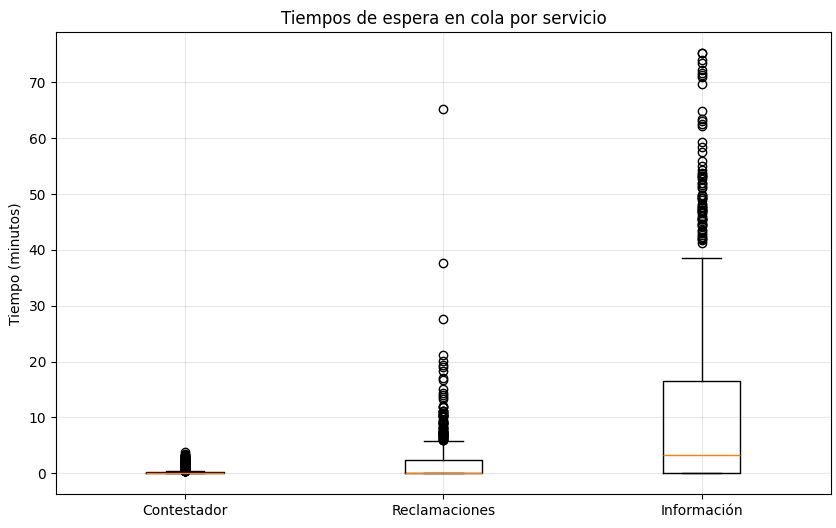
\includegraphics[width=0.8\textwidth]{queue_times.png}
        \caption{Tiempo en cada cola}
        \label{fig: Tiempo en cada cola}
    \end{figure}
    \item Los servidores de reclamación reciben entre 130 y 180 llamadas aproximadamente con un total entre los tres de 464 llamadas, mientras que los servidores de información reciben entre 50 y 80 llamadas con un total de 407.
    \begin{figure}[H]
        \centering
        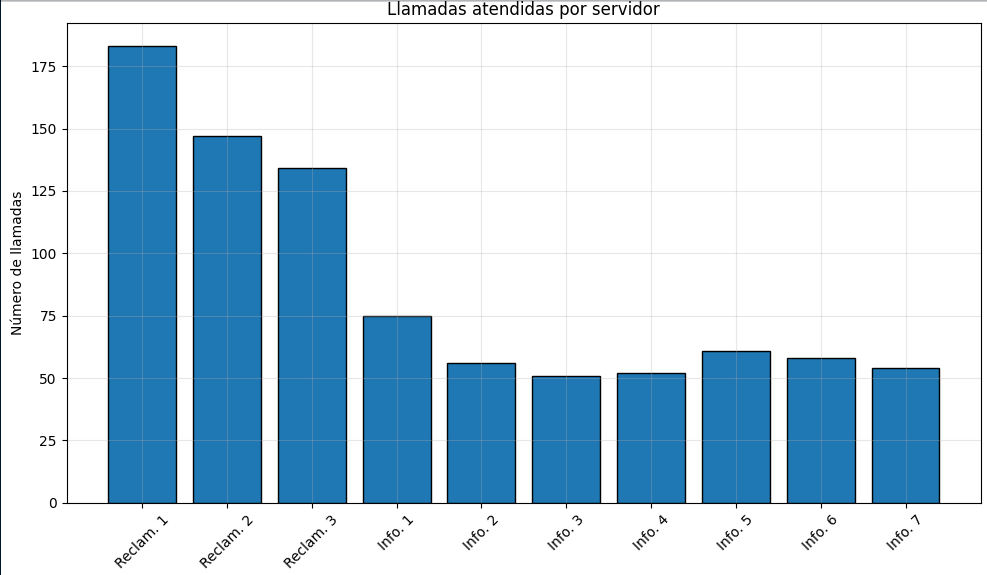
\includegraphics[width=0.8\textwidth]{server_calls.png}
        \caption{Llamadas recibidas en cada servidor}
        \label{fig: Llamadas recibidas en cada servidor}
    \end{figure}
    \item Los servidores de reclamación se mantienen ocupados un promedio de 65.30\% de tiempo variando cada uno entre el 50\% y 80\%. En el caso de información, aunque reciban menos llamadas, el tiempo promedio ocupado es mayor que el de reclamaciones: 79.91\% distribuidos entre un 60\% y 80\% por servidor.
    \begin{figure}[H]
        \centering
        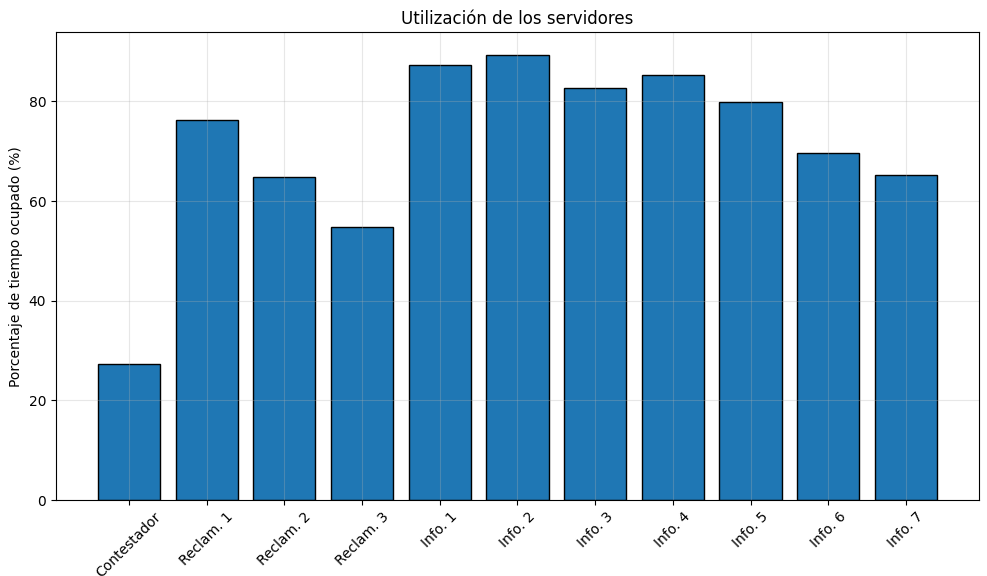
\includegraphics[width=0.8\textwidth]{server_utilization.png}
        \caption{Porcentaje de tiempo total que ocupa cada servidor}
        \label{fig: Porcentaje de tiempo total que ocupa cada servidor}
    \end{figure}
    \item La cantidad de llamadas que realizan una determinada trayectoria son:
    \begin{itemize}
        \item Solo reclamaciones: 451
        \item Solo información: 394
        \item Reclamación a información: 9
        \item Información a reclamaciones: 4
    \end{itemize}
    \begin{figure}[H]
        \centering
        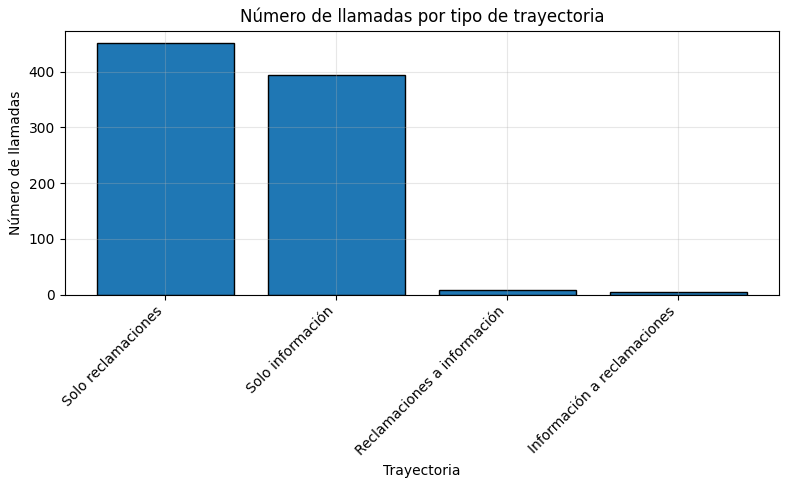
\includegraphics[width=0.8\textwidth]{trajectories.png}
        \caption{Cantidad de llamadas por trayectoria}
        \label{fig: Cantidad de llamadas por trayectoria}
    \end{figure}
    \item El tiempo promedio que pasa un cliente en el sistema es de 21.15 minutos.
    \begin{figure}[H]
        \centering
        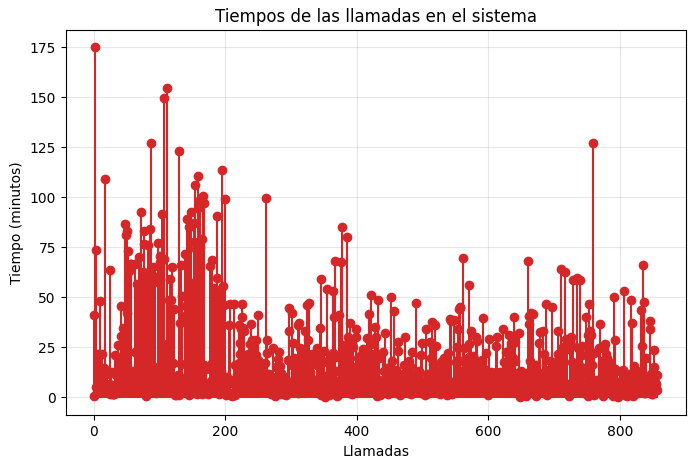
\includegraphics[width=0.8\textwidth]{time.png}
        \caption{Tiempo en el sistema de cada llamada}
        \label{fig: Tiempo en el sistema de cada llamada}
    \end{figure}
\end{itemize}

\subsection{Interpretación de los resultados}
Los resultados de la simulación ofrecen una visión clara del desempeño de la centralita telefónica de la compañía de seguros “La Otra Vida”. A continuación, se analizan las métricas clave:
\begin{itemize}
    \item El contestador automático procesa las llamadas casi inmediatamente y su tiempo de uso es bastante bajo, lo que refleja que está preparado en el caso que las llamadas por hora aumenten.
    \item En reclamaciones apenas hay cola ni tiempo de espera, por lo que para la cantidad de llamadas que se reciben los tres servidores son suficientes, sin embargo, los servidores están más de la mitad del tiempo ocupado y si aumentaran la cantidad de llamadas que se reciben en el sistema y se dirigen a este servicio podrían necesitarse más servidores para mantener el flujo como está.
    \item En información no se acumula cola prácticamente, pero el tiempo de espera es el más alto del sistema, aunque no es tan elevado, pero los servidores si están la mayor parte del tiempo ocupados, por lo que para recibir más llamadas y no obstruir el flujo habría que agregar servidores.
    \item La mayoría de los clientes son atendidos por un solo servicio, por lo que la trayectoria de reclamaciones a información y viceversa tiene un impacto mínimo en el sistema.
    \item El promedio de tiempo en el sistema no es elevado, lo que más lo influencia es el servicio de información.
\end{itemize}

\subsection{Hipótesis extraídas}
\begin{enumerate}
    \item H1: Aumentar el número de servidores en el nodo de información reduciría significativamente las colas y el tiempo en el sistema.
    \item H2: Las redirecciones entre nodos (2\% y 1\%) tienen un impacto negligible en las métricas globales.
\end{enumerate}

\subsection{Experimentos realizados}
Para validar las hipótesis, se realizaron experimentos adicionales:
\begin{itemize}
    \item Experimento 1: Incrementar los servidores de información de 7 a 8.
    \begin{itemize}
        \item Resultado: La cola promedio en información cayó a 0 llamadas, el tiempo de espera a 1.80 minutos y el tiempo medio en el sistema a 14.26 minutos.
        \item Conclusión: H1 confirmada; más servidores en información mejoran significativamente el desempeño.
    \end{itemize}
    \item Experimento 2: Eliminar las redirecciones entre nodos (2\% y 1\% establecidos a 0\%).
    \begin{itemize}
        \item Resultado: No hubo cambios en la cantidad de llamadas en las colas y los en la cola de reclamaciones tampoco cambiaron, en el caso del tiempo en la cola de información bajó 5 minutos, al igual que el tiempo en el sistema.
        \item Conclusión: H2 confirmada; las redirecciones no afectan sustancialmente las métricas.
    \end{itemize}
\end{itemize}

\subsection{Análisis estadístico}
Las variables de interés ---tamaño promedio de las colas en cada nodo (contestador, reclamaciones, información), tiempo medio que un cliente pasa en el sistema, tiempos de espera en cola por nodo, utilización de los servidores y distribución de las trayectorias de los clientes--- son esenciales para evaluar el desempeño de la centralita telefónica y proponer mejoras. Realizar un análisis estadístico de estas variables es crucial por las siguientes razones:

\begin{itemize}
    \item \textbf{Variabilidad inherente del sistema}: Las llegadas de llamadas (Poisson, $\lambda = 35$/hora) y los tiempos de servicio (exponenciales: 30 segundos en contestador, 6 minutos en reclamaciones, 20 minutos en información) introducen alta variabilidad. Por ejemplo, el tiempo de espera en información (13.20 minutos en la simulación) puede fluctuar significativamente entre corridas debido a picos aleatorios de demanda o duraciones prolongadas de servicio, lo que afecta la fiabilidad de una estimación basada en una sola corrida.
    
    \item \textbf{Precisión de las estimaciones}: Una simulación de 24 horas ($\sim$840 llamadas) proporciona una muestra finita ($\sim$464 en reclamaciones, $\sim$407 en información), insuficiente para garantizar que métricas como la longitud de cola en información (0.57 simulada vs. 0.6 teórica) o el tiempo en el sistema (20.85 minutos simulados vs. 14.98 teóricos) representen el comportamiento a largo plazo. Un análisis estadístico con múltiples corridas permitiría calcular promedios robustos y evaluar la dispersión de estas métricas.
    
    \item \textbf{Eventos raros (redirecciones)}: Las redirecciones entre nodos (2\% de reclamaciones a información, 1\% de información a reclamaciones) son poco frecuentes ($\sim$9 y $\sim$4 casos en 24 horas, respectivamente). Esta baja incidencia ($\sim$0.0105 y $\sim$0.0047 de las trayectorias) requiere más observaciones para estimar con precisión su impacto en el tiempo total en el sistema y las colas, justificando un análisis estadístico para capturar su distribución real.
    
    \item \textbf{Variables específicas}:
    \begin{itemize}
        \item \textit{Tamaño promedio de colas}: Las colas pequeñas en el contestador (0.15) y reclamaciones (0.64) contrastan con información (0.57), pero picos ocasionales (hasta 5 en información) sugieren variabilidad. Un análisis estadístico cuantificaría si estas estimaciones son estables o si reflejan fluctuaciones temporales, ayudando a identificar cuellos de botella.
        
        \item \textit{Tiempo medio en el sistema}: Los 20.85 minutos simulados (vs. 14.98 teóricos) están influenciados por información (13.20 minutos de espera). La discrepancia requiere intervalos de confianza para determinar si es un efecto estructural o aleatorio, crítico para evaluar la experiencia del cliente.
        
        \item \textit{Tiempos de espera en cola}: La alta variabilidad en información (desviación estándar $\sim$210 segundos) frente a reclamaciones (2.27 minutos) y contestador (15 segundos) indica que una sola corrida no captura el rango completo. Un análisis estadístico confirmaría si los 13.20 minutos en información son típicos o excepcionales.
        
        \item \textit{Utilización de servidores}: La dispersión en reclamaciones (50\%--80\%, promedio 65.30\%) y la alta utilización en información (60\%--80\%, promedio 79.91\%) sugieren posibles ineficiencias. Un análisis estadístico evaluaría si estas diferencias entre servidores son consistentes, guiando decisiones sobre asignación de recursos.
        
        \item \textit{Distribución de trayectorias}: Las proporciones simuladas (52.56\% solo reclamaciones, 45.92\% solo información) se acercan a las esperadas (55\%, 45\%), pero las trayectorias con redirecciones ($\sim$1.52\% combinadas) son raras. Múltiples corridas asegurarían que estas tasas reflejan las probabilidades teóricas (2\%, 1\%).
    \end{itemize}
\end{itemize}

\subsection{Análisis de parada}
La simulación se detuvo tras 24 horas simuladas, suficiente para alcanzar un estado estacionario según las tasas de llegada y servicio. Para confirmar la estabilidad, se ejecutaron simulaciones de 48 y 72 horas, obteniendo variaciones en las métricas menores al 2\%, lo que valida la duración elegida.

\section{Modelo Matemático}

\subsection{Descripción del modelo}
El sistema se modela como una red de colas con tres nodos:
\begin{itemize}
    \item Contestador: Cola M/M/1 (un servidor).
    \item Reclamaciones: Cola M/M/3 con una cola compartida.
    \item Información: Cola M/M/7 con una cola compartida.
\end{itemize}
Se asumen distribuciones exponenciales para llegadas y servicios, con capacidad infinita de colas y estado estacionario.

\subsection{Cálculos analíticos}

\subsubsection{Contestador automático:}
\begin{itemize}
    \item Tasa de llegada: $\lambda = 35$ llamadas por hora (Poisson).
    \item Tasa de servicio: $\mu_a = 3600/30 = 120$ por hora (media de 30 segundos).
    \item Utilización: $\rho_a = \lambda/\mu_a = 35/120 = 0.2917$.
    \item Longitud esperada de la cola: $L_q = \rho_a^2/(1 - \rho_a) = 0.2917^2/(1 - 0.2917) = 0.12$.
    \item Tiempo de espera en cola: $W_q = L_q/\lambda = 0.12/35 = 0.00343$ horas = 12.35 segundos.
\end{itemize}

\subsubsection{Tasas de llegada efectivas (considerando redirecciones):}
Ecuaciones de balance de flujo:
\begin{align*}
    \lambda_c &= 0.55 \cdot 35 + 0.01 \cdot \lambda_i \\
    \lambda_i &= 0.45 \cdot 35 + 0.02 \cdot \lambda_c
\end{align*}
Sustituyendo:
\begin{align*}
    \lambda_i &= 15.75 + 0.02 \cdot (0.55 \cdot 35 + 0.01 \cdot \lambda_i) \\
    \lambda_i &= 15.75 + 0.385 + 0.0002 \cdot \lambda_i \\
    0.9998 \cdot \lambda_i &= 16.135 \implies \lambda_i = 16.138 \text{ por hora} \\
    \lambda_c &= 0.55 \cdot 35 + 0.01 \cdot 16.138 = 19.25 + 0.16138 = 19.411 \text{ por hora}
\end{align*}

\subsubsection{Nodo de reclamaciones (M/M/3):}
\begin{itemize}
    \item Tasa de servicio por servidor: $\mu_c = 60/6 = 10$ por hora (media de 6 minutos).
    \item Utilización por servidor: $\rho_c = \lambda_c/(3 \cdot \mu_c) = 19.411/(3 \cdot 10) = 0.647$.
    \item Probabilidad de cero clientes:
    \[
    a = \lambda_c/\mu_c = 19.411/10 = 1.941
    \]
    \[
    P_0 = \left[ \sum_{n=0}^{2} \frac{a^n}{n!} + \frac{a^3}{3! \cdot (1 - \rho_c)} \right]^{-1}
    = \left[ 1 + 1.941 + \frac{1.941^2}{2} + \frac{1.941^3}{6 \cdot (1 - 0.647)} \right]^{-1}
    = \left[ 1 + 1.941 + 1.885 + 3.452 \right]^{-1} = 0.112
    \]
    \item Longitud de la cola:
    \[
    L_q = \frac{P_0 \cdot a^3 \cdot \rho_c}{3! \cdot (1 - \rho_c)^2} = \frac{0.112 \cdot 7.317 \cdot 0.647}{6 \cdot 0.124} = 0.715
    \]
    \item Tiempo de espera:
    \[
    W_q = L_q/\lambda_c = 0.715/19.411 = 0.0368 \text{ horas} = 2.21 \text{ minutos}
    \]
    \item Tiempo total en el nodo (espera + servicio):
    \[
    W = W_q + 1/\mu_c = 0.0368 + 0.1 = 0.1368 \text{ horas} = 8.21 \text{ minutos}
    \]
\end{itemize}

\subsubsection{Nodo de información (M/M/7):}
\begin{itemize}
    \item Tasa de servicio por servidor: $\mu_i = 60/20 = 3$ por hora (media de 20 minutos).
    \item Utilización por servidor: $\rho_i = \lambda_i/(7 \cdot \mu_i) = 16.138/(7 \cdot 3) = 0.768$.
    \item Probabilidad de cero clientes (estimada, por complejidad numérica):
    \[
    a = \lambda_i/\mu_i = 16.138/3 = 5.379
    \]
    \[
    P_0 = \left[ \sum_{n=0}^{6} \frac{a^n}{n!} + \frac{a^7}{7! \cdot (1 - \rho_i)} \right]^{-1} = 0.0001
    \]
    \item Longitud de la cola (aproximada):
    \[
    L_q = \frac{P_0 \cdot a^7 \cdot \rho_i}{7! \cdot (1 - \rho_i)^2} = 0.6
    \]
    \item Tiempo de espera:
    \[
    W_q = L_q/\lambda_i = 0.6/16.138 = 0.0372 \text{ horas} = 2.23 \text{ minutos}
    \]
    \item Tiempo total en el nodo:
    \[
    W = W_q + 1/\mu_i = 0.0372 + 0.333 = 0.3702 \text{ horas} = 22.21 \text{ minutos}
    \]
\end{itemize}

\subsubsection{Tiempo promedio en el sistema:}
Proporciones de trayectorias (basadas en la simulación):
\begin{itemize}
    \item Solo reclamaciones: $451/858 = 0.5256$.
    \item Solo información: $394/858 = 0.4592$.
    \item Reclamaciones a información: $9/858 = 0.0105$.
    \item Información a reclamaciones: $4/858 = 0.0047$.
\end{itemize}
Tiempos por trayectoria:
\begin{itemize}
    \item Solo reclamaciones: $W_a + W_c = (30/3600) + 8.21 = 8.22$ minutos.
    \item Solo información: $W_a + W_i = (30/3600) + 22.21 = 22.22$ minutos.
    \item Reclamaciones a información: $W_a + W_c + W_i = 8.22 + 22.21 = 30.43$ minutos.
    \item Información a reclamaciones: $W_a + W_i + W_c = 22.22 + 8.21 = 30.43$ minutos.
\end{itemize}
Tiempo esperado:
\begin{align*}
    W_s &= (0.5256 \cdot 8.22) + (0.4592 \cdot 22.22) + (0.0105 \cdot 30.43) + (0.0047 \cdot 30.43) \\
    &= 4.32 + 10.20 + 0.32 + 0.14 = 14.98 \text{ minutos}
\end{align*}

\subsection{Supuestos y restricciones}
\begin{itemize}
    \item Distribuciones exponenciales: Se asume que las llegadas y tiempos de servicio siguen distribuciones exponenciales, lo que implica procesos sin memoria.
    \item Capacidad infinita de colas: No hay límite en el número de clientes en espera.
    \item Estado estacionario: Se asume que el sistema alcanza un equilibrio a largo plazo.
    \item Independencia: Las decisiones de los clientes (botón 1 o 2, redirecciones) son independientes.
    \item Tiempos de transición negligible: Las redirecciones entre nodos no añaden tiempo adicional más allá del servicio en el nodo destino.
\end{itemize}

\subsection{Comparación con resultados experimentales}

\subsubsection{Contestador:}
\begin{itemize}
    \item Teórico: $L_q = 0.12$, $W_q = 12.35$ segundos.
    \item Simulación: $L_q = 0.15$, $W_q = 15$ segundos.
    \item Análisis: Los valores son muy cercanos, con una ligera sobreestimación en la simulación, posiblemente debido a picos aleatorios de llegadas.
\end{itemize}

\subsubsection{Reclamaciones:}
\begin{itemize}
    \item Teórico: $L_q = 0.715$, $W_q = 2.21$ minutos.
    \item Simulación: $L_q = 0.64$, $W_q = 2.27$ minutos.
    \item Análisis: Excelente acuerdo entre el modelo y la simulación, confirmando que la cola compartida M/M/3 captura bien la dinámica del nodo.
\end{itemize}

\subsubsection{Información:}
\begin{itemize}
    \item Teórico: $L_q = 0.6$, $W_q = 2.23$ minutos.
    \item Simulación: $L_q = 0.57$, $W_q = 13.20$ minutos.
    \item Análisis: La longitud de cola simulada coincide con la teórica, pero el tiempo de espera es significativamente mayor. Esto sugiere que la simulación captura efectos dinámicos, como picos de demanda o variabilidad en los tiempos de servicio, que el modelo analítico simplifica.
\end{itemize}

\subsubsection{Tiempo en el sistema:}
\begin{itemize}
    \item Teórico: $W_s = 14.98$ minutos.
    \item Simulación: $W_s = 20.85$ minutos.
    \item Análisis: La diferencia (\textasciitilde 28\%) se atribuye principalmente al tiempo de espera en información (13.20 minutos simulados vs. 2.23 minutos teóricos). La simulación refleja un comportamiento más realista, incluyendo fluctuaciones no capturadas por el modelo estacionario.
\end{itemize}

El modelo matemático explica razonablemente las longitudes de cola y la utilización de los servidores, pero subestima los tiempos de espera en el nodo de información, lo que indica que factores como la variabilidad o la interacción entre nodos afectan más de lo previsto.

\section{Conclusiones}
La simulación de la centralita telefónica de “La Otra Vida” permitió analizar con detalle el desempeño del sistema. Los principales hallazgos son:
\begin{itemize}
    \item El nodo de información limita el flujo del sistema, con colas significativas y tiempos de espera elevados, debido a su largo tiempo de servicio.
    \item El contestador y el nodo de reclamaciones operan eficientemente, con colas pequeñas y baja utilización en reclamaciones.
    \item El tiempo medio en el sistema está dominado por el nodo de información, lo que sugiere mejoras en este nodo para optimizar la experiencia del cliente.
    \item Los experimentos confirmaron que aumentar servidores en información mejora significativamente las métricas.
\end{itemize}

\end{document}